% Generated from: Zhihu/专栏：概率与统计/渐近统计 (5)：Delta 方法_金鱼马_2026-04-23.md
在参数估计中，一个常见的情境是：对参数 $\theta\in\mathbb R^k$，我们有一列估计量 $\{T_n\}_{n=1}^\infty$，并且知道其渐近性质，如
\[
T_n\overset{P}\longrightarrow\theta,
\qquad
\sqrt n(T_n-\theta)\overset{\rm d}\longrightarrow F.
\]

但现在我们关心的不是 $\theta$ 本身，而是它的一个函数 $\phi(\theta)$，其中 $\phi:\mathbb R^k\to\mathbb R^m$。比如，$\theta$ 是正态分布的方差，我们想要估计标准差 $\sqrt\theta$；或者 $\theta$ 是两点分布的参数 $p$，我们想要估计对数几率 $\log\tfrac p{1-p}$。朴素的想法是直接用 $\phi(T_n)$ 去估计 $\phi(\theta)$，那么 $\phi(T_n)$ 的渐近分布是什么？这就是 Delta 方法回答的问题。

\section{一阶 Delta 方法}

如果 $\phi$ 是连续的，那么由连续映射定理，$T_n\overset{P}\to\theta\implies \phi(T_n) \overset{P}\to \phi(\theta)$，但这没有提供 $\phi(T_n)$ 渐近分布的信息。我们想知道的是
\[\sqrt n(\phi(T_n)-\phi(\theta))\overset{\rm d}\to \;?\]
直觉上，如果 $\phi$ 足够光滑，那么在 $\theta$ 附近， $\phi(T_n)$ 可以近似为 $\phi(\theta) + \phi'(\theta)(T_n-\theta)$。于是 $\sqrt{n}(\phi(T_n)-\phi(\theta))$ 应该近似于 $\phi'(\theta) \sqrt{n}(T_n-\theta)$，它的极限分布就是 $\phi'(\theta)F$ 。这个想法非常的简单，但非常有效。

Delta 方法本质上就是这样的一套基于 Taylor 展开的``分布传播''技术，它告诉我们在何种条件下，估计量的渐近分布和收敛速度能够被光滑变换所保持。

我们将这一想法正式地整理为定理，记 $\phi'(\theta)\in\mathbb R^{m\times k}$ 是 $\phi$ 在 $\theta$ 处的 Jacobian 矩阵，

\begin{theorem}[一阶 Delta 方法]\label{thm:ch5:first-order-delta}

设 $\phi$ 在 $\theta$ 处可微，且 $\phi'(\theta)\neq 0$；估计量 $T_n$ 满足 $a_n(T_n-\theta)\overset{\rm d}\to F$。

其中 $\{a_n\}$ 是确定的数列，有 $a_n\to \infty$。那么

\begin{enumerate}
\def\labelenumi{\arabic{enumi}.}
\tightlist
\item
  $a_n\big(\phi(T_n)-\phi(\theta)\big) - \phi'(\theta)\big(a_n(T_n-\theta)\big) \overset{P}\to 0$ ；
\item
  $a_n\big(\phi(T_n)-\phi(\theta)\big) \overset{\rm d}\to \phi'(\theta)\,F$ 。
\end{enumerate}

\end{theorem}

\begin{proof}

可微性告诉我们 $R(h):=\phi(\theta+h)-\phi(\theta)-\phi'(\theta)h=o(\|h\|)$。由 $a_n(T_n-\theta)\overset{\rm d}\to F$ 和 $a_n\to\infty$ 知 $T_n-\theta \overset{P}\to 0$，根据第~\ref{ch:random-convergence}~章的引理~\ref{lem:ch1:stochastic-plugin}，我们可将上式的 $h$ 替换为 $T_n-\theta$；再乘以 $a_n$ 即可得到
\[
\begin{aligned}
&a_n\bigl(\phi(T_n)-\phi(\theta)\bigr)
-\phi'(\theta)a_n(T_n-\theta)\\
&\qquad=o_P(a_n\|T_n-\theta\|)
=o_P(O_P(1))=o_P(1).
\end{aligned}
\]
这就证明了 (1.)。(2.) 直接由 Slutsky 定理（推论~\ref{cor:ch1:slutsky}）即得：\\\[a_n\big(\phi(T_n)-\phi(\theta)\big) = \phi'(\theta)\big(a_n(T_n-\theta)\big) + o_P(1) \overset{\rm d}\to \phi'(\theta)F\]
\end{proof}

最简单的例子是 $F$ 为正态分布的情形：

\begin{corollary}\label{cor:ch5:delta-normal}
设 $\theta\in \mathbb R^k$ 的估计量 $T_n$ 满足渐近正态性 $\sqrt n(T_n-\theta)\overset{\rm d}\to \mathcal N(0,\Sigma)$，其中 $n\to\infty$，

其中 $\Sigma\succeq 0$ 是 $k\times k$ 方阵。那么对可微函数 $\phi:\mathbb R^k\to\mathbb R^m$ ， $\phi'(\theta)\ne 0$ ，有
\[\sqrt n\big(\phi(T_n)-\phi(\theta)\big)\overset{\rm d}\to \mathcal N\big(0,\phi'(\theta)\Sigma\phi'(\theta)^\top \big)\]\end{corollary}

\section{二阶 Delta 方法}

一阶 Delta 方法很大程度上依赖于 $\phi'(\theta)\ne 0$ ；如果这一条件不满足，我们需要利用更高阶的 Taylor 展开。设 $\phi'(\theta)=0$ 但 Hessian $\phi''(\theta)\ne 0$ ，那么
\[\phi(T_n)=\phi(\theta)+\frac12\phi''(\theta)(T_n-\theta)^2+\cdots\]
那么应有
\[n\big(\phi(T_n)-\phi(\theta)\big)=\frac12\phi''(\theta)\big(\sqrt n(T_n-\theta)\big)^2\overset{\rm d}\to \frac12\phi''(\theta)F^2\]
一个很常见的情形是 $\sqrt n\bar X_n\overset{\rm d}\to \mathcal N(0,1)$ ，那么对于这样的 $\phi$ ， $n\phi(\bar{X}_n)\overset{\rm d}\to \frac12\phi''(\theta)\chi_1^2$ 。可以看到，在一阶方法中，我们乘以的系数是 $\sqrt n$ ；而在二阶方法中，由于一阶导数消失，主导项变成了二次项，我们需要乘以 $n$ 才能得到非退化的分布，这也意味着，当 $\phi'(\theta)=0$ 时， $\phi(T_n)$ 收敛到 $\phi(\theta)$ 的速度要更快。

\begin{example}[余弦变换的二阶 Delta 方法]
设 i.i.d. 随机变量 $X_1,\dots,X_n$ 有均值 0 和方差 $\sigma^2$ ，则中心极限定理告诉我们 $\sqrt{n}\bar{X}_n \overset{\rm d}\to \mathcal{N}(0,\sigma^2)$。考虑 $\phi(x)=\cos x$，在 $\theta=0$ 处 $\phi'(0)=-\sin 0 =0$，$\phi''(0)=-\cos 0 = -1$。于是
\[
-2n(\cos\bar{X}_n - 1) \overset{\rm d}\to \big(\mathcal{N}(0,\sigma^2)\big)^2 = \sigma^2 \chi_1^2.
\]

\end{example}

\begin{example}[Bernoulli 分布的 Kullback--Leibler 散度]\label{ex:ch5:bernoulli-kl}
分布 $P_\theta$ 到 $P_\eta$ 的 Kullback--Leibler（KL）散度定义为
\[
D_{\mathrm{KL}}(P_\theta\Vert P_\eta)
:=\mathbb E_\theta\left[\log\frac{p_\theta(X)}{p_\eta(X)}\right],
\qquad X\sim P_\theta,
\]
其中 $p_\theta$ 与 $p_\eta$ 分别是 $P_\theta$ 与 $P_\eta$ 的密度函数。
设 $X_1,\ldots,X_n$ i.i.d. 服从参数为 $\theta\in(0,1)$ 的 Bernoulli 分布，
$\widehat\theta_n=\bar X_n$。那么，
\[
nD_{\mathrm{KL}}(P_\theta\Vert P_{\widehat\theta_n})
\overset{\rm d}\longrightarrow \frac12\chi_1^2.
\]
\begin{proof}
Bernoulli 分布的概率质量函数为
$p_\theta(x)=\theta^x(1-\theta)^{1-x}$，其中 $x\in\{0,1\}$，因而
\[
\begin{aligned}
D_{\mathrm{KL}}(P_\theta\Vert P_{\widehat\theta_n})
&=\mathbb E_\theta\left[
  \log\frac{p_\theta(X)}{p_{\widehat\theta_n}(X)}
\right]\\
&=\theta\log\frac\theta{\widehat\theta_n}
 +(1-\theta)\log\frac{1-\theta}{1-\widehat\theta_n}.
\end{aligned}
\]
对 $t\in(0,1)$ 定义
\[
f(t):=\theta\log\frac\theta t
+(1-\theta)\log\frac{1-\theta}{1-t}.
\]
其前两阶导数为
\[
f'(t)=-\frac\theta t+\frac{1-\theta}{1-t},
\qquad
f''(t)=\frac\theta{t^2}+\frac{1-\theta}{(1-t)^2}.
\]
所以 $f(\theta)=f'(\theta)=0$，且
$f''(\theta)=1/[\theta(1-\theta)]$。由二阶 Delta 方法，
\[
\begin{aligned}
n\bigl(f(\widehat\theta_n)-f(\theta)\bigr)
&=\frac12f''(\theta)
  \bigl(\sqrt n(\widehat\theta_n-\theta)\bigr)^2+o_P(1)\\
&=\frac12\left(
  \frac{\sqrt n(\widehat\theta_n-\theta)}
       {\sqrt{\theta(1-\theta)}}
\right)^2+o_P(1)\\
&\overset{\rm d}\longrightarrow \frac12\chi_1^2,
\end{aligned}
\]
其中最后一步使用了 Bernoulli 样本均值的中心极限定理。
% 证明嵌在例子内，结尾仅保留 example 环境的一个方块。
\let\endproof\par
\end{proof}
\end{example}


当然，我们还可以向更高次项展开，单变量和多变量 $\phi$ 的情况分别如下：

\begin{theorem}[高阶 Delta 方法（一维）]\label{thm:ch5:higher-order-delta-univariate}

设 $\phi:\mathbb R\to \mathbb R$ 是单变量函数，在 $\theta\in\mathbb R$ 处 $r$ 次可微，且导数满足
\[
\phi^{(j)}(\theta)=0,\; j=1,\dots,r-1,\quad \phi^{(r)}(\theta)\neq 0.
\]

若估计量 $T_n$ 满足 $a_n(T_n-\theta)\overset{\rm d}\to F$，则
\[
\frac{a_n^{r}\big(\phi(T_n)-\phi(\theta)\big)}{\frac{1}{r!}\phi^{(r)}(\theta)} \overset{\rm d}\to F^r,\quad \text{ 当 }n\to\infty.
\]

\end{theorem}

\begin{theorem}[高阶 Delta 方法（多维）]\label{thm:ch5:higher-order-delta-multivariate}

设 $\phi:\mathbb R^k\to\mathbb R$ ，在 $\theta\in\mathbb R^k$ 处 $r$ 次可微，且所有 $1$ 阶到 $r-1$ 阶的偏导数在 $\theta$ 处均为零：
\[\frac{\partial^j\phi  (\theta)}{\partial x_{i_1}\cdots \partial x_{i_j}}=0,\quad 1\le j\le r-1,\forall i_1,\ldots,i_j\in\{1,\ldots,k\}\]
但 $r$ 阶偏导数不全为零，即存在某个 $(i_1,\dots,i_r)$ 使得
\[
\frac{\partial^r \phi (\theta)}{\partial x_{i_1}\cdots\partial x_{i_r}} \neq 0.
\]

若估计量 $T_n$ 满足 $a_n(T_n-\theta)\overset{\rm d}\to F=(F_1,\dots,F_k)$ ，则
\[a_n^{r}\,\big(\phi(T_n) - \phi(\theta)\big) \overset{\rm d}\to \frac{1}{r!}\sum_{i_1=1}^k \cdots \sum_{i_r=1}^k \left( \frac{\partial^r \phi (\theta)}{\partial x_{i_1}\cdots\partial x_{i_r}} \cdot \prod_{j=1}^r F_{i_j}\right),\quad \text{ 当 }n\to\infty.\]\end{theorem}

例如，可参考 \cite{serfling1980}, \S3.3, Theorem B。

这些结论都很复杂，在实际统计应用中很少出现。

\section{Delta 方法的例子}

下面我们通过几个经典统计例子，展示 Delta 方法的实际使用。

\subsection{样本方差的渐近正态性}

第一个例子，我们考察样本方差 $S_n:=\frac1n\sum_{i=1}^n(X_i-\bar{X})^2$ 的渐近分布。

\begin{example}[样本标准差的渐近分布]\label{ex:ch5:sd-variance}
设 $X_1,\dots,X_n$ i.i.d. 取值总体 $X$ 。记

\begin{itemize}
\tightlist
\item
  总体 $r$ 阶原点矩为 $\alpha_r:=\mathbb{E}[X^r]$ ，特别地，总体均值为 $\alpha_1$ ；
\item
  样本 $r$ 阶原点矩为 $a_{r,n}:=\frac1n\sum_{i=1}^nX_i^r$ ，特别地，样本均值为 $\bar{X}_n=a_{1,n}$ ；
\item
  总体 $r$ 阶中心矩为 $\mu_r:=\mathbb{E}[(X-\alpha_1)^r]$ ，特别地，总体方差为 $\mu_2$ 。
\end{itemize}

设总体的四阶矩存在。根据多维的中心极限定理，我们知道
\[ \sqrt{n}\begin{pmatrix} a_{1,n}-\alpha_1 \\ a_{2,n}-\alpha_2 \end{pmatrix} \overset{\rm d}\to \mathcal{N}\left(0, \mathrm{Var}\left[\begin{pmatrix} X \\ X^2 \end{pmatrix}\right]\right),\quad \text{ 当 }n\to\infty \]

另一方面，样本方差可写作 
\[ S_n := \frac1n\sum_{i=1}^n (X_i-\bar{X}_n)^2 = a_{2,n} - a_{1,n}^2 \]
考虑函数 $\phi(x_1,x_2)=x_2-x_1^2$ ，Jacobi 矩阵为 $\phi'(\alpha_1,\alpha_2) = (-2\alpha_1,\, 1)^\top\ne 0$，因此由 Delta 方法， $\sqrt{n}(S_n - \mu_2)$ 依分布收敛于正态分布 $\mathcal N(0,\Sigma)$ ，其中，
\[\begin{aligned} \Sigma&=(-2\alpha_1,1)\mathrm{Var}\left[\begin{pmatrix}X_1\\ X_1^2\end{pmatrix}\right]\begin{pmatrix}-2\alpha_1\\ 1\end{pmatrix}\\ &=\mathrm{Var}[-2\alpha_1X_1+X_1^2]\\ &=\mathrm{Var}[(X_1-\alpha_1)^2]\\ &=\mu_4-\mu_2^2 \end{aligned}\]
即，
\[\sqrt n(S_n-\mu_2)\overset{\rm d}\to \mathcal N(0,\mu_4-\mu_2^2),\quad \text{ 当 }n\to\infty\]

当然，我们知道 $S_n$ 是 $\mu_2$ 的有偏估计量，而 $s_n:=\frac n{n-1}S_n=\frac1{n-1}\sum_{i=1}^n(X_i-\bar{X})^2$ 才是无偏估计。注意到$\frac{n}{n-1}=1+\frac{1}{n-1}$，则
\[\sqrt{n}(s_{n}-\mu_2) = \sqrt{n}(S_n-\mu_2) + \underbrace{\frac{\sqrt{n}}{n-1}S_n}_{o_P(1)}\]
因此 $s_n$ 和 $S_n$ 有相同的渐近分布。

此外，如果我们考虑样本标准差 $\sqrt {S_n}$ ，则可直接对 $\phi(x)=\sqrt x$ 用 Delta 方法，由 $\phi'(\mu_2)=\frac1{2\sqrt{\mu_2}}$ 有
\[\sqrt n(\sqrt{S_n}-\sqrt{\mu_2})\overset{\rm d}\to \mathcal N\left(0,\frac{\mu_4-\mu_2^2}{4\mu_2}\right),\quad \text{ 当 }n\to\infty\]\end{example}

\subsection{渐近正态的变换}

\begin{example} \label{ex:ch5:asymptotic-normal}
设 $X_n$ 满足 $\frac{X_n-\mu}{\sigma_n^2}\overset{\rm d}\to \mathcal N(0,1)$ ，其中 $\sigma_n\to 0$ ，我们常简记为 $X_n \sim AN(\mu,\sigma_n^2)$。利用一阶 Delta 方法，有以下变换成立：

\begin{itemize}
\tightlist
\item
  $X^2_n \sim AN(\mu^2,4\mu^2\sigma_n^2)$ ，其中 $\mu\ne 0$ 。
\item
  $X_n^{-1}\sim AN(\mu^{-1},\mu^{-4}\sigma_n^2)$ ，其中 $\mu\ne 0$ 。
\item
  $e^{X_n}\sim AN(e^\mu,e^{2\mu}\sigma_n^2)$ 。
\item
  $\log |X_n|\sim AN(\log |\mu|,\mu^{-2}\sigma_n^2 )$ ，其中 $\mu\ne 0$ 。
\end{itemize}
\end{example}


值得注意的是，在例~\ref{ex:ch5:asymptotic-normal} 的第一条里，若 $\mu=0$ ，那么结论相应地要改成 $X_n^2/\sigma_n^2 \to \chi_1^2$ 。这可以推广到高维，见下例，


\begin{example}[二次型的 Delta 方法]
设 $k$ 维随机向量 $X_1,\dots,X_n$ i.i.d. ，总体有均值 $\mu$ 和协方差矩阵 $\Sigma$ ；多维中心极限定理告诉我们 \[ \sqrt{n}(\bar{X}-\mu)\overset{\rm d}\to \mathcal N_k(0,\Sigma) \]下面考察 $\phi(\bar{X})=\bar{X}^\top \bar X$ ，若 $\mu\ne 0$ ，那么 $\phi'(\mu)=2\mu$ ，故
\[\sqrt n\Big(\bar{X}^\top\bar{X}-\mu^\top\mu\Big)\overset{\rm d}\to \mathcal N(0,(2\mu)^\top\Sigma(2\mu))=\mathcal N(0,4\mu^\top\Sigma\mu)\]
当 $\mu=0$ 时又如何呢？，因为 $\sqrt{n}\bar{X} \overset{\rm d}\to \mathcal{N}_k(0,\Sigma)$，所以
\[n\bar{X}^\top\bar{X} \overset{\rm d}\to Z^\top \Sigma Z,\]
其中 $Z\sim\mathcal{N}(0,\mathbf I_k)$。这是一个加权 χ² 分布：若 $\Sigma = U^\top \operatorname{diag}(\lambda_1,\dots,\lambda_p)U$，则
\[
Z^\top\Sigma Z \overset{\rm d}= \sum_{i=1}^k \lambda_i \chi_{1i}^2.
\]

这里 $\chi_{1i}^2$ 独立同分布于 $\chi_1^2$。

由此，还可以看到收敛速度

\begin{itemize}
\tightlist
\item
  当 $\mu\ne 0$ 时， $\bar{X}^\top\bar{X}-\mu^\top\mu=O_P(1/\sqrt n)$ ；
\item
  当 $\mu=0$ 时， $\bar{X}^\top\bar{X}=O_P(1/n)$ 。
\end{itemize}
\end{example}

\subsection{方差的 χ² 检验}

\begin{example}[方差的 χ² 检验]
设 $X_1,\dots,X_n$ i.i.d. 同分布于 $\mathcal{N}(\mu,\sigma^2)$ ，其中 $\mu\in\mathbb R$ 、 $0<\sigma^2<\infty$ 未知。有如下检验问题
\[H_0:\sigma^2\le 1 \quad \iff\quad H_1:\sigma^2>1\]
在正态总体下，$\frac{nS_n}{\sigma^2}\sim\chi_{n-1}^2$。因此，可以，我们可以用如下检验统计量
\[\sum_{i=1}^n(X_i-\bar{X})^2=nS_n\]
记 $\chi^2_{n-1}(\alpha)$ 为 $\chi^2_{n-1}$ 的 $\alpha$ 分位数，那么以 $\{nS_n\le \chi^2_{n-1}(1-\alpha)\}$ 作为接受域，该检验的功效满足
\[\begin{aligned} P(nS_n>\chi^2_{n-1}(1-\alpha)\mid \sigma^2\le 1)&=P\left(\frac{nS_n}{\sigma^2}>\frac{\chi^2_{n-1}(1-\alpha)}{\sigma^2}\Big|\,\sigma^2\le 1\right)\\ &\le P(\chi^2_{n-1}>\chi^2_{n-1}(1-\alpha))\\ &=\alpha \end{aligned}\]
于是该检验有水平 $\alpha$ ，这便是我们熟知的 χ² 检验。

然而，χ² 检验对正态性十分敏感。若总体是某个非正态分布 $F$ ，应该怎么办？

\end{example}

\begin{example} 
设 $F$ 有均值 $\mu$ 和方差 $\sigma^2$ ，四阶矩存在，记 $\kappa := \frac{\mathbb{E}[(X-\mu)^4]}{\sigma^4}-3$ 为峰度，并设 $\kappa>0$ 。

一方面，用前文例~\ref{ex:ch5:sd-variance} 的结论， \[ \sqrt n\left(\frac {S_n}{\sigma^2}-1\right)\overset{\rm d}\to \mathcal N(0,\kappa+2) \]另一方面，我们知道，对于 $Z_1,\dots,Z_{n-1}\sim \mathcal N(0,1)$ i.i.d. 有 $\sum_{i=1}^{n-1}Z_i^2\sim\chi_{n-1}^2$ ，从而中心极限定理告诉我们\[ \frac{\chi_{n-1}^2-(n-1)}{\sqrt{2(n-1)}}\overset{\rm d}\to \mathcal N(0,1),\quad \text{ 当 }n\to\infty \]若以 $\xi_{1-\alpha}$ 记标准正态分布的上 $\alpha$ 分位数，则
\[\begin{aligned} & P\left(\frac{\chi_{n-1}^2-(n-1)}{\sqrt{2(n-1)}}\ge \xi_{1-\alpha}\right)\to P(\mathcal N(0,1)\ge \xi_{1-\alpha})= \alpha = P(\chi_{n-1}^2\ge \chi^2_{n-1}(1-\alpha))\\ \implies &\chi_{n-1}^2(\alpha)\approx (n-1)+\sqrt{2(n-1)}\xi_{1-\alpha}  \end{aligned}\]
从而，如果仍然直接采用 χ² 检验，我们将得到功效
\[\begin{aligned} P\Big(nS_n>\chi_{n-1}^2(1-\alpha)\Big|\,\sigma^2\le 1 \Big)&=P\left(\sqrt n\left(\frac{S_n}{\sigma^2}-1\right)>\frac{\chi^2_{n-1}(1-\alpha)-n}{\sqrt n}\,\Bigg|\,\sigma^2\le 1\right)\\ &\approx P\left(\sqrt n\left(\frac{S_n}{\sigma^2}-1\right)>\frac{(n-1)+\sqrt{2(n-1)}\xi_{1-\alpha}-n}{\sqrt n}\,\Bigg|\,\sigma^2\le 1\right)\\ &\to P\Big(\mathcal N(0,\kappa+2)>\sqrt 2\xi_{1-\alpha}\Big)\\ &=1-\Phi\left(\frac{\sqrt 2\xi_{1-\alpha}}{\sqrt{\kappa+2}}\right)\\ &>1-\Phi(\xi_{1-\alpha})=\alpha\\ \end{aligned}\]
因此 χ² 检验不再有水平 $\alpha$ 。

当然，在大样本下，χ² 检验仍然是有用的，因为我们同时可以看出当备择假设 $H_1$ 成立（ $\sigma^2>1$ ）时，
\[\begin{aligned} P( nS_n > \chi^2_{n-1}(1-\alpha)\mid \sigma^2 > 1 ) &= P  \left( \sqrt{n} \left( \frac{S_n}{\sigma^2} - 1 \right) > \frac{\sigma^{-2} \chi^2_{n-1}(1-\alpha)-n}{\sqrt{n}}\bigg| \sigma^2 > 1 \right)\\  &\approx P\left(\mathcal{N}(0, \kappa + 2) > \frac{\sigma^{-2}\big((n-1) + \xi_{1-\alpha} \sqrt{2(n-1)}\big) - n}{\sqrt{n}}\right)\\  &= 1 - \Phi\left(\frac{(\sigma^{-2} - 1)\sqrt{n}}{\sqrt{\kappa + 2}} - \frac{\sigma^{-2}}{\sqrt{n(\kappa + 2)}} + \frac{\sqrt{2}\,\xi_{1-\alpha}}{\sqrt{\kappa + 2}}\sqrt{\frac{n-1}{n}}\right)\\  &\approx 1 - \Phi\left(\frac{(\sigma^{-2} - 1)\sqrt{n}}{\sqrt{\kappa + 2}} + \frac{\sqrt{2}}{\sqrt{\kappa + 2}}\xi_{1-\alpha}\right) \\ &\to 1 \end{aligned}\]
因此 χ² 检验是相合的，即，当备择假设成立时，随着样本量增大，检验几乎一定能拒绝原假设。
\end{example}

\subsection{多项分布拟合优度检验}
 
\begin{example}[Pearson $\chi^2$ 统计量]
设有多项分布 $(n_1,\dots,n_K) \sim \text{Multinomial}(n;\,p_1,\dots,p_K)$，$p_i>0$。设经过 $n$ 次 i.i.d. 抽样后，有实际频数为 $n_i$ 、频率 $\widehat{p}_i := n_i/n$，则由多元中心极限定理，
\[X_n := \sqrt{n}\bigl(\widehat{p}_1-p_1,\dots,\widehat{p}_K-p_K\bigr)^\top \overset{\rm d}\to \mathcal{N}_K(0,\Sigma)\]
其中 $\Sigma = (\sigma_{ij})_{k\times k}$ 是协方差矩阵：
\[\begin{aligned} \sigma_{ij}&=\begin{cases} p_i(1-p_i),&\text  {若 }i=j\\ -p_ip_j,&\text{ 若 }i\ne j \end{cases}\\ &=p_i(\delta_{ij}-p_j) \end{aligned}\]
Pearson χ² 拟合优度检验采用如下检验统计量：
\[
T_n := \sum_{i=1}^K \frac{(n_i-np_i)^2}{np_i} = n\sum_{i=1}^K \frac{1}{p_i}(\widehat{p}_i-p_i)^2 = X_n^\top C X_n.
\]

其中 $C := \operatorname{diag}(p_1^{-1},\dots,p_K^{-1})$ 。根据连续映射定理，该统计量有极限
\[T_n \overset{\rm d}\to Z^\top \Sigma^{1/2} C \Sigma^{1/2} Z\]
其中 $Z\sim \mathcal N_K(0,\mathbf I_K)$ 。注意到 $\Sigma^{1/2}C\Sigma^{1/2}$ 是秩为 $K-1$ 的幂等矩阵：

\begin{itemize}
\tightlist
\item
  $(C\Sigma)_{ij} = \sum_{l} C_{il} \sigma_{lj} = p_i^{-1} \sigma_{ij} = p_i^{-1} \cdot p_i(\delta_{ij}-p_j) = \delta_{ij} - p_j$ ，于是 $(C\Sigma)^2_{ij} = \sum_l (\delta_{il}-p_l)(\delta_{lj}-p_j)=\delta_{ij}-p_j=(C\Sigma)_{ij}$ ，说明 $C\Sigma$ 幂等。
\item
  从而，与之相似的 $\Sigma^{1/2}C\Sigma^{1/2} = \Sigma^{1/2} (C\Sigma) \Sigma^{-1/2}$ 也是幂等矩阵。
\item
  其秩为 $\mathrm{tr}(A) = \mathrm{tr}(C\Sigma)=\sum_i (C\Sigma)_{ii} = \sum_i (\delta_{ii} - p_i) = \sum_i (1 - p_i) = K - 1$ 。
\end{itemize}

故 $T_n \overset{\rm d}\to \chi_{K-1}^2$，这是 Pearson χ² 检验的基本理论依据。
\end{example}
注意到 Pearson 统计量不是一个对称的统计量，这里的``不对称''指的是，它不是一个``实际频率'' $\widehat p_i$ 和``理论频率'' $p_i$ 的对称函数，因而也无法视作两个分布的``度量 (metric)''。不过，我们可以利用 Delta 方法对它进行改造：对 $\phi(x)=\sqrt x$ 用定理~\ref{thm:ch5:first-order-delta} 的第 (1.) 条，得到
\[
\sqrt n\big(\sqrt{\widehat{p_i}}-\sqrt{p_i}\big)
-\frac1{2\sqrt{p_i}}\sqrt n(\widehat p_i-p_i)
\overset{P}\to 0.
\]
于是
\[
4n\big(\sqrt{\widehat p_i}-\sqrt{p_i}\big)^2
=n\frac{(\widehat p_i-p_i)^2}{p_i}+o_P(1).
\]
这说明如下的统计量与 Pearson $\chi^2$ 检验的统计量 $T_n$ 有相同的渐近分布：
\[
T^{(g)}_n
=4n\sum_{i=1}^K(\sqrt{\widehat p_i}-\sqrt{p_i})^2
=:8nH^2(\widehat p,p).
\]
这被称作 Hellinger 统计量，其中
\[
H(\widehat p,p)
:=\sqrt{\frac12\sum_{i=1}^K(\sqrt{\widehat{p}_i}-\sqrt{p_i})^2}
=\sqrt{1-\sum_{i=1}^K\sqrt{\widehat{p}_ip_i}}
\]
是 \emph{\textbf{Hellinger 距离}}。它关于 $p_i$ 和 $\widehat p_i$ 是对称的，且取值位于 0 到 1 之间；相比于 Pearson $\chi^2$ 检验，Hellinger 距离往往拥有更好的鲁棒性。

\subsection{Wald 检验}\label{ex:ch5:wald-test}
 

\begin{example}[Wald 检验]
设有 i.i.d. $k$ 维随机向量 $X_1,X_2,\dots,X_n\sim F$ ，总体有均值 $\mu$ 和协方差矩阵 $\Sigma$ 。考虑如下双边检验问题：
\[
H_0:\mu=\mu_0\quad \iff \quad H_1:\mu\ne \mu_0.
\]

假设如下条件成立：

\begin{itemize}
\tightlist
\item
  总体 $F$ 的协方差矩阵满秩： $\Sigma\succ 0$ ；
\item
  样本的协方差矩阵 $S_n:=\frac1n\sum_{i=1}^n(X_i-\bar{X})(X_i-\bar{X})^\top$ 总满秩： $S_n\succ 0$ 。
\end{itemize}

那么，根据大数律， $S_n\overset{P}\to \Sigma$ 且 $S_n^{-1}\overset P\to \Sigma^{-1}$ 。

Wald 检验提出使用如下统计量：
\[
W_n:=n(\bar X_n-\mu_0)^\top S_n^{-1}(\bar{X}_n-\mu_0).
\]

注意到当原假设 $H_0$ 成立时：
\[\begin{aligned} W_n &= \sqrt{n}(\bar{X}-\mu_0)^\top \Sigma^{-1} \sqrt{n}(\bar{X}-\mu_0)  + \sqrt{n}\underbrace{(\bar{X}-\mu_0)^\top}_{O_P(n^{-1/2})}\underbrace{ (S_n^{-1}-\Sigma^{-1}) }_{o_P(1)}\sqrt{n}\underbrace{(\bar{X}-\mu_0) }_{O_P(n^{-1/2})}\\ &= \sqrt{n}(\bar{X}-\mu_0)^\top \Sigma^{-1} \sqrt{n}(\bar{X}-\mu_0)  +  o_P(1) \end{aligned}\]
以及 $\sqrt n\Sigma^{-1/2}(\bar{X}-\mu_0)\overset{\rm d}\to\mathcal N_k(0,\mathbf I_k)$ ，可知 $W_n\overset{\rm d}\to \chi_k^2$ ，于是可将 $\{W_n\le \chi^2_k(1-\alpha)\}$ 作为接受域。
\end{example}
Delta 方法允许我们将这套方法用在非线性假设上面： 
$$H_0:g(\mu)=0\quad \iff \quad H_1:g(\mu)\ne 0$$

其中 $g:\mathbb R^k\to\mathbb R^m$ 连续可微，且 Jacobian 矩阵 $g'(\mu)$ 总有秩 $m$ 。那么，我们可以使用如下检验统计量 

$$W_n:=ng(\bar{X})^\top\bigl(g'(\bar X)S_n g'(\bar X)^\top\bigr)^{-1}g(\bar{X})$$

由 Delta 方法，在 $H_0$ 下， 

$$\sqrt ng(\bar{X})=\sqrt n(g(\bar{X})-g(\mu))\overset{\rm d}\to \mathcal N_m\bigl(0,g'(\mu)\Sigma g'(\mu)^\top\bigr)$$

同时连续映射定理告诉我们 $g'(\bar X)S_n g'(\bar X)^\top\overset{P}\to g'(\mu)\Sigma g'(\mu)^\top$ ，再由 Slutsky 定理，立即得到 $W_n\overset{\rm d}\to \chi_m^2$

这个框架的核心是将非线性约束 $g(\theta)=0$ 通过 Delta 方法线性化，它使得我们可以把 Wald 检验用在更广泛的假设检验问题上（不局限于均值参数），设有检验问题： 
$$H_0:\theta\in\Theta_0\quad \iff\quad H_1:\theta\in\Theta\setminus\Theta_0$$

其中参数空间 $\Theta$ 是 $\mathbb R^k$ 中有内点的子集， $\Theta_0\subset \Theta$ 是一个 $k-m$ 维子流形（ $m\le k$ ），使得我们可以用 $\Theta_0=\{\theta\in\Theta:g(\theta)=0\}$ 对原假设进行刻画。
 

\begin{theorem}[Wald 统计量的渐近分布]
\label{thm:ch5:wald-asymptotic-distribution}
设
\begin{itemize}
\tightlist
\item
  $g:\Theta\to\mathbb R^m$ 连续可微，在参数空间上其 Jacobian $g'(\theta)$ 总有秩 $m$ ；
\item
  $\theta$ 有一个渐近正态估计 $\widehat\theta_n$ 使得 $a_n(\widehat\theta_n-\theta)\overset{\rm d}\to \mathcal N_k(0,\Sigma)$ ；
\item
  $\Sigma\succ 0$ ，并且存在一个相合估计使得 $\widehat \Sigma_n\overset{P}\to \Sigma$ ，同时（至少当 $n$ 充分大时） $\widehat \Sigma_n\succ 0$ 。
\end{itemize}

那么 Wald 统计量 \[ W_n=a_n^2g\big(\widehat\theta_n\big)^\top \Big(g'\big(\widehat\theta_n\big)\widehat\Sigma_ng'\big(\widehat\theta_n\big)^\top\Big)^{-1}g\big(\widehat\theta_n\big) \]就有极限分布 $\chi_m^2$ 。

\end{theorem}

\begin{remark}

\begin{itemize}
\tightlist
\item
  在一定的正则条件下，极大似然估计 (MLE) 就是渐近正态的： $\sqrt n\big(\widehat\theta_n-\theta\big)\overset{\rm d}\to \mathcal N(0,I(\theta)^{-1})$ 所以往往取 $\widehat\theta_n$ 为 MLE。上式中 $I(\theta)$ 是总体分布的 Fisher 信息矩阵，用样本 Fisher 信息矩阵估计之。可见~\ref{sec:ch7:wald-test} 节。
\item
  这里的某些条件是可以放松的，如矩阵不可逆时能用广义逆取代 (\cite{andrews1987})。
\end{itemize}
\end{remark}

\section{方差稳定变换}

在已知估计量 $T_n$有渐近分布 \[ \sqrt n(T_n-\theta)\overset{\rm d}\to \mathcal N(0,\sigma^2) \]之后，我们往往就会利用它计算置信区间，或者进行假设检验。以置信区间为例，取 \[ \texttt{CI}_n=\left[T_n-\xi_{1-\alpha/2}\frac{\sigma^2}{\sqrt n},T_n+\xi_{1-\alpha/2}\frac{\sigma^2}{\sqrt n}\right] \]就近似有置信水平 $\alpha$ 。

然而这里的渐近方差 $\sigma^2=\sigma^2(\theta)$ 往往依赖于 $\theta$，这意味着我们基于 $T_n$ 的渐近分布算出的置信区间，宽度会随 $\theta$ 变化，这往往会带来麻烦。\textbf{\emph{方差稳定变换 }} (Variance Stabilizing Transformation, VST) 的思想是：找到一个变换 $\phi$，使得 $\phi(T_n)$ 的渐近方差为常数 $c^2$（与 $\theta$ 无关）。

由 Delta 方法（简单起见，这里假设 $\phi$ 是映射到 $\mathbb R$ 的连续函数， $\phi'(\theta)\ne 0$ ），
\[\sqrt{n}(\phi(T_n)-\phi(\theta)) \overset{\rm d}\to \mathcal{N}\bigl(0,\,(\phi'(\theta))^2\sigma^2(\theta)\bigr)\]
我们希望 $(\phi'(\theta))^2\sigma^2(\theta)=c^2$，即
\[\phi'(\theta) = \frac{c}{\sigma(\theta)} \quad \Longrightarrow \quad \phi(\theta) = c\int \frac{{\rm d}\theta}{\sigma(\theta)}\]
常数 $c$ 可以任意选取（通常取 $c=1$ 或 $c$ 使得变换后方差为 1）。

\begin{example}[Fisher's $z$-transformation]\label{ex:ch5:fisher-z}
设 $(X_1,Y_1),(X_2,Y_2),\dots$ i.i.d. 同分布于二维正态分布，总体相关系数为 

$$\rho = \frac{\mathrm{Cov}[X,Y]}{\sqrt{\mathrm{Var}[X]\,\mathrm{Var}[Y]}} = \frac{\mathbb{E}[(X-\mu_X)(Y-\mu_Y)]}{\sigma_X\,\sigma_Y}$$ 

样本相关系数定义为
\[
r_n:={\frac {\sum _{i=1}^n(X_i-{\bar {X}})(Y_i-{\bar {Y}})}{{\sqrt {\sum _{i=1}^n(X_i-{\bar {X}})^2}}{\sqrt {\sum _{i=1}^n(Y_i-{\bar {Y}})^2}}}}.
\]
可以证明 $r$ 是 $\rho$ 的渐近正态估计：
\[
\sqrt{n}(r_n - \rho) \overset{\rm d}\to\mathcal N(0, (1-\rho^2)^2).
\]

% 具体过程比较繁琐，从略。可见

% \href{https://www.zhihu.com/question/51402458/answer/1975264119998394908}{the delta method 是干什么的？}

则 VST 是
\[
\phi(\rho)=\int\frac1{1-\rho^2}\mathrm d\rho=\frac12\log\frac{1+\rho}{1-\rho}=\operatorname{arctanh} \rho.
\]
从而
\[
\sqrt n\Big(\operatorname{arctanh}r_n-\operatorname{arctanh} \rho\Big)\overset{\rm d}\to\mathcal N(0,1).
\]

对任意的 $\rho$ 成立。据此可以构造出近似的 $\alpha$ 置信区间 \[ \left(\tanh \left(\operatorname{arctanh} r_n-\frac{\xi_{1-\alpha/2}}{\sqrt n}\right),\tanh \left(\operatorname{arctanh} r_n+\frac{\xi_{1-\alpha/2}}{\sqrt n}\right)\right) \]这种``取样本相关系数 arctanh''的方法叫做 \href{https://en.wikipedia.org/wiki/Fisher_transformation}{Fisher z-变换}。图~\ref{fig:ch5:fisher-z-transform} 给出了一个例子：对相关系数 $\rho=0.5$ 的总体重复模拟 $10^5$ 次，每次使用 12 个独立样本计算 $r_n$，并分别绘制 Fisher 变换之前（左）和之后（右）的直方图。可以看到，除了稳定方差外，Fisher $z$-变换的另一优点是将分布对称化。

\begin{figure}[htbp]
  \centering
  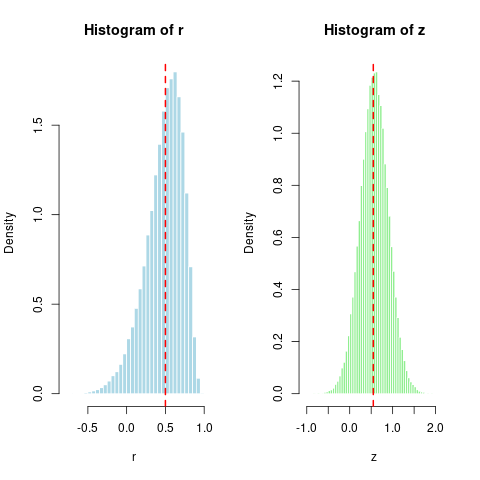
\includegraphics[width=0.62\textwidth]{figures/05-fisher-z-transform.png}
  \caption{Fisher $z$-变换前后的模拟分布（R 绘制）}
  \label{fig:ch5:fisher-z-transform}
\end{figure}

\begin{verbatim}
m = 10^5; r=numeric(m);  n = 12
 for(i in 1:m) {
    u1 = rnorm(n); u2 = rnorm(n);  u3=rnorm(n)
    x = u1 + u2;  y = u2 + u3
    r[i] = cor(x, y) }

summary(r); sd(r)
## Min. 1st Qu.  Median    Mean 3rd Qu.    Max. 
## -0.7282  0.3429  0.5176  0.4822  0.6590  0.9804 
## 0.23916

# Fisher z transformation
z <- 0.5 * log((1 + r) / (1 - r))

summary(z); sd(z)
## Min. 1st Qu.  Median    Mean 3rd Qu.    Max. 
## -0.9248  0.3573  0.5731  0.5746  0.7910  2.3083 
## 0.3310624
\end{verbatim}


\end{example}

\begin{example}[Tukey's Hanging Rootgram]
设 i.i.d. 随机变量 $X_1,X_2,\dots,X_n\sim F$ ，有密度函数 $f$ 。\textbf{\emph{核密度估计 }} (KDE) 或者称 Parzen-Rosenblatt 密度估计如下：
\[\widehat{f}_{nh}(x) = \frac{1}{nh}\sum_{i=1}^n K\!\left(\frac{x-X_i}{h}\right)\]
其中 $K$ 是核函数（满足适当正则条件），如标准正态密度； $h=h(n)$ 是平滑带宽。

有这样的结论 \cite{parzen1962}：若平滑带宽满足：当 $n\to\infty$ 时， $nh\to \infty$ 但 $nh^5\to 0$，那么KDE 有渐近正态性：
\[
\sqrt{nh}\big(\widehat f_{nh}(x)-f(x)\big)\overset{\rm d}\to \mathcal N\left(0, {\textstyle f(x)\int K^2(y){\rm d}y}\right).
\]

因此 $\widehat{f}_{nh}(x)\sim AN\left(f(x), \textstyle{\frac{\int K^2(y){\rm d}y}{nh}f(x)}\right)$ ，忽略掉常数，其渐近方差依赖于 $f(x)$ 。于是 VST 可以取
\[
\phi(f) =\frac12 \int \frac{{\rm d}f}{\sqrt{f}} = f^{1/2}.
\]
从而，对 $\big(\widehat{f}_{nh}(x)\big)^{1/2}$ ，有
\[
\big(\widehat{f}_{nh}(x)\big)^{1/2}\sim AN\left(f(x), \frac{\int K^2(y){\rm d}y}{4nh}\right).
\]

\end{example}

关于密度估计，有一本经典的参考教材 \cite{silverman1986}，介绍得十分详尽。

% 最后要说的是，在现代统计学中，由于 Bootstrap（自助法）的普及，我们往往可以直接通过重采样来计算复杂置信区间。但除了构建置信区间，VST 还有两个重要作用：一是满足经典模型（如方差分析、线性回归）的同方差性假设；二是去除估计量方差与均值的耦合关系，使得我们可以更客观地比较不同总体的离散程度。
